% !TEX root = ../proj_report_outline.tex

\chapter{Proposed Architectures}\label{C:arch}
In this chapter we use the intuitions gathered from related works to propose novel classes of
architectures employing tensor decompositions to implement multiplicative connections. There are
two key principles: simplicity and modularity. We want to design networks that have no extraneous
components, such that every element of the network has a clearly defined role.

\section{Incorporating tensors for expressivity}
We have established that incorporating tensors into networks is a promising line of inquiry, all that
remains is how precisely to formulate it.

\subsection{Biases}
Neural networks typically require biases to be able to express a full range of transformations. We would
expect a tensor layer to be no different. A common way to conceptualise the addition of a bias for a
given layer is to incorporate it into the weight matrix by adding an additional row and inserting a
corresponding input which has its value fixed to one. With a bilinear product gives more than
just the addition of a bias vector. We use \(\tilde{\phantom{x}}\) to represent altering the inputs
and weights in this way: \(\tilde{\vec{x}}\) is an input vector with an additional \(1\) appended
and \(\tilde{\mat{U}}\) is a matrix with a corresponding additional row.

Generalising this construction to a three-way tensor we have to take an \(n_1 \times n_2 \times n_3\)
tensor to a \(n_1 + 1 \times n_2 \times n_3 +1\). This leads to the addition of a vector as well as
two more matrix products. For a three-way tensor \(\tensor{W}\),
\begin{equation}\label{eq:tensorbias}
	\tran{\tilde{\vec{x}}}\widetilde{\tensor{W}}\tilde{\vec{y}}
	= \tran{\vec{x}}\tensor{W}\vec{y} + \mat{U}\vec{y} + \mat{V}\vec{x} + \vec{b}.
\end{equation} This is very similar to the manner in which the states are computed in the vanilla
RNN, just with the addition of the multiplicative tensor interactions.

Applying the same process when the tensor is represented in the CP decomposition does not
have the same result. Instead it simply results in adding bias vectors to two of the internal
matrix products. Let \(\tensor{W} = [A, B, C]_{CP}\), then simply appending ones to the inputs
results in
\begin{equation}
	\tran{\tilde{\vec{x}}}\widetilde{\tensor{W}}\tilde{\vec{y}}
	= \tran{\mat{B}}\left( (\mat{A}\vec{x} + \vec{b}_x) \odot (\mat{C}\vec{y} + \vec{b}_y)\right).
\end{equation} This is quite different to equation~\eqref{eq:tensorbias} meaning that if we wish to
insert such a tensor product into a neural network we must choose whether to leave the biases in
the decomposition or treat the bias matrices separately. The latter provides less control over the
parameters, as there are now two matrices unaffected by the rank, but it might be helpful in that we
could use a very low rank decomposition and still maintain a baseline behaviour.

\subsection{Generalised Multiplicative RNN}\label{sec:gmrnn}
The simplest architecture way to incorporate a decomposed tensor is to use it to generalise the
Multiplicative RNN and Multiplicative Integration RNN \autocite{Martens2011a, Wu2016}.
To do this, we simply replace the various linear operations with a bilinear form with appropriate
biases:
\begin{equation}\label{eq:gmrnn}
	\vec{h}_t = \tau\left( \tran{\tilde{\vec{x}}_t}\tilde{\tensor{W}}\tilde{\vec{h}}_{t-1} \right)
\end{equation}
Choosing to keep the biases elements separate from the decomposition gives a form which captures
vanilla RNNs as well as several types of multiplicative RNNs:
\begin{equation}\label{eq:gmrnnbias}
	\vec{h}_t = \tau\left(\tran{\vec{x}_t}\tensor{W}\vec{h}_{t-1}
		+ \mat{U}\vec{h}_{t-1} + \mat{V}\vec{x}_t + \vec{b}\right).
\end{equation} We term this the Generalised Multiplicative RNN (GMR). Unfortunately this
network will still exhibit the same vanishing gradients as the vanilla RNN as the state updates
still pass through a matrix (albeit one modulated by the new input).

\section{Gates and Long Time Dependencies}
To address these vanishing gradients, we turn to the same solution as the LSTM and GRU: an additive state
update. A naive purely additive state update would solve the issues with the gradient vanishing, but
causes a number of other issues. A better method is to use a \emph{gated} recurrence. The LSTM and
the GRU both use such a method to produce new states, but they differ slightly. We investigate
the implications of both schemes and decide that the scheme employed in the GRU has appealing 
properties which allow us to design simple yet flexible architectures with well defined components.

\subsection{Naive Addition}\label{sec:additive}
The simplest possible approach is to have the network compute a candidate vector of hidden states
\(\vec{z}_t\) and compute new hidden states as
\begin{equation}\label{eq:additiveupdate}
	\vec{h}_t = \vec{h}_{t-1} + \vec{z}.
\end{equation}

Recalling equation~\eqref{eq:bptt-v}, the problematic term was \(\nabla_{\vec{h_{k-1}}}\vec{h}_k\),
the gradient of a hidden state with respect to its immediate precursor. If the state is computed by
equation~\eqref{eq:additiveupdate}:
\begin{equation}
	\nabla_{\vec{h}_{k-1}}\vec{h}_k = \mat{I} + \nabla_{\vec{h}_{k-1}}\vec{z}_k.
\end{equation} Adding the identity matrix ensures the eigenvalues of the gradient are at least
one, which negates the potential to vanish.

While the gradients will not vanish, they may still explode. Pascanu et al. show that a necessary
condition for exploding gradients, when using the hyperbolic tangent activation, is that the largest
eigenvalue of the recurrent weight matrix is greater than one \autocite{Pascanu2012}. This is shown by
observing that the \(l2\) norm of the gradient\footnote{
The \(l2\) norm of a matrix is the norm induced by the \(l2\) norm on vectors:\\
\(||\mat{A}||_2 = \sup \left\{||\mat{Ax}||_2: \vec{x} \in \mathbb{R}^n, ||\vec{x}||_2 = 1 \right\}\)
which turns out to be the square root of the largest eigenvalue.} is upper bounded by the product of the
norms of the recurrent weight matrices and the gradient of the nonlinearity. For our purposes it suffices
to observe the eigenvalues of the gradient with this additive scheme are always at least one, so unless
the other component is zero, the gradients must necessarily explode.

With care and gradient clipping \autocite{Pascanu2012} exploding gradients can be managed, but there
is a more intuitive reason why this network is naive: a purely additive
network will struggle to forget. At each step, it will always add to the current state. Therefore,
the candidate state must contain negative values to ever remove any information from the state. This
suggests two things: the candidate state must depend on the previous state (so that it knows what to
remove) and that the network will need to be very precise with its scale so that it can
actually remove information that is no longer necessary. This last point suggests that the network
will have trouble if the non-linearity applied to the candidate states is bounded -- if it erroneously
adds during training it will struggle to learn to subtract. An unbounded non-linearity would likely
exacerbate the gradient issues, which makes this sort of a network challenging to design.


\subsection{Gates}\label{sec:gate}
LSTMs and GRUs manage their additive connections by applying multiplicative gates. We will therefore
investigate the solutions they present, with a view to choosing the best. We refer to the LSTM's gate
as a \emph{forget} gate, which is consistent with the literature. This type performs best
 in the presence of other gates \autocite{Greff2016, Jozefowicz2015}, which is explained by our 
 theoretical analysis.
The gate on the GRU is slightly
different and has a number of advantageous properties. We term this the \emph{convex} gate and find it
is sufficiently flexible to allow us to remove the dependency of the candidate state on the hidden
state, which is desirable in terms of simplifying the architecture as well as controlling the gradients.

Before delving into their specific properties, we first describe the gating mechanisms.
Denote by \(p_t\) the gate signal at time \(t\) (which is a
function of both the input and the current state and bounded in \([0, 1]\)). We also use
\(h_t\) to refer to the hidden state at time \(t\), the object of interest, and \(z_t\) will
refer to the candidate update computed by the rest of the network. In general these
elements will be vectors, but in the following we assume scalars with no loss of generality as
the vector forms contain only element-wise operations.

We can define the
forget gate's recurrence as
\begin{equation}
	h_t = p_th_{t-1} + z_t
	\label{eq:forgetgate}
\end{equation} for \(z_t\) the new candidate state which is typically a function of
both \(h_{t-1}\) and the input at time \(t\). This allows the network to wholly replace the
state with a new value, but as will be shown in detail it has no control over the incoming
flow of information. For exact equivalence with the LSTM, it suffices to note that the \(z_t\)
could be computed in any way, including with its own gating mechanisms.

The convex gate makes the following modification:
\begin{equation}
	h_t = p_th_{t-1} + (1-p_t)z_t.
	\label{eq:cvexgate}
\end{equation} This allows the one gate signal
to control the acceptance or rejection of new information.

In order to analyse the possible behaviours of these gates, we observe that each state \(h_t\)
can be expanded as a weighted sum over all \(z_i\) for \(i < t\). In this sense, we can think of
the states as being a sliding-window sum over candidates where the shape of the window is defined
recursively by the \(p_i\) values.\footnote{There is in fact no sliding window -- the sum is always
over all values. However given the range of window shapes the gating mechanism is capable of producing
it is reasonable to think about it as something close to a one-dimensional convolution.}
With this view in mind, we note that we can think of the
gate signals \(p_i\) as providing an \emph{attention} mechanism which controls how the network
attends to the information from past time steps.

\subsubsection{Forget Gate}
The forget gate is designed to allow the network to completely replace a state, hence its name.
Clearly for this to happen the gate signal simply needs to be zero. Further, the default behaviour
is to pay more attention to recently acquired information. If we define the initial
state \(h_0 = 0\), we can rewrite the first few states as
\begin{align}
	h_1 &= z_1 \\
	h_2 &= p_2z_1 + z_2 \\
	h_3 &= p_3h_2 + z_3 \\
		&= p_3(p_2z_1 + z_2) + z_3 \\
		&= p_3p_2z_1 + p_3z_2 + z_3
\end{align} In general,
\begin{equation}
	h_t = \sum_{i=1}^{t-1} \left(\prod_{j=i+1}^t p_j\right) \cdot z_i + z_t.
\end{equation} Each state is a weighted sum of the past states, with strictly
non-increasing weights as we go back in time.
Note that the coefficient of each past candidate is the product over all gate signals from the
current time back to the candidate in question. As the gate signals are in \([0, 1]\), 
this is likely to correspond to a very steep decay.


Figure~\ref{fig:lstmgates} shows some consequences of this scheme. It is clear
that it offers a blunt choice -- exponential decay over time or accumulating all states from a
 certain point nearly equally. This means that the mechanism for
producing candidate states is very important. 

Consider the case where the network needs to remember an event from one time step some time in the
past and ignore all further input. Achieving this with the forget gate can be done in two
ways. Firstly, the gate values can be clamped to one and the
candidates to zero. Clamping the gates to one produces a rectangular window; the state will be an
evenly weighted sum of all candidates from the point the gate switches on. If the goal is to pick
out a single candidate and remember it for a long time, all subsequent
candidates will have to be zero. 
The second method of remembering a single candidate state is by keeping the exponential window 
and simply producing the same candidate at every future time step (with
appropriate scaling).

Both of these require a significant degree of co-operation between the gate and the mechanism that
produces candidate activations. Further, the production of candidate activations has to be quite
flexible and most likely depend on the previous state. The LSTM achieves this with further gating
of inputs and outputs, enabling the candidate to depend heavily on previous states. We hypothesise that
having to learn this degree of co-operation hinders learning by gradient descent as it requires a
carefully tuned balance to be maintained through the training process or gradients will vanish or
explode.


\begin{figure}[t]
\centering
\begin{subfigure}[t]{0.45\textwidth}
	\centering
	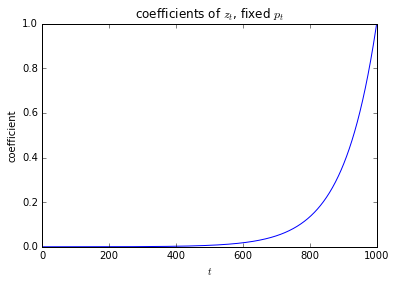
\includegraphics[width=\textwidth]{newarchs/lstmexp}
	\caption{Coefficients of \(z_t\) resulting from a fixed, high value of all \(p_t\)
	under the forget gate scheme.}
\end{subfigure}~
\begin{subfigure}[t]{0.45\textwidth}
	\centering
	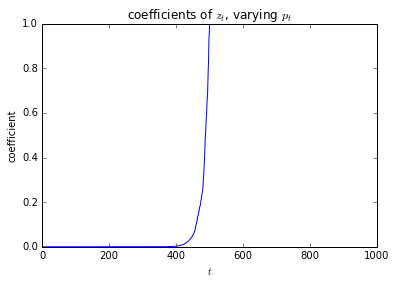
\includegraphics[width=\textwidth]{newarchs/lstmrect}
	\caption{Coefficients of \(z_t\) random \(p_t\) up to \(t=500\) and all \(p_t\) after
	500 set to 1.}
\end{subfigure}
\caption[Forget gate window shapes]
{Different window shapes produced by the forget gate. As each coefficient at time \(t\)
is the product of all gate values from \(t\) down to 1, the range of possible shapes is limited.}
\label{fig:lstmgates}
\end{figure}

The shape of this window affects access to past information which can be an issue during training. 
Intuitively it would be good for the
information stored in the states to persist so that its presence will affect the gradients being
back-propagated which will affirm or suppress its presence. This is going to be an issue when
the newly accumulated information decays away exponentially in time, as will be the case early on
when the gate values will be essentially random. A solution to this issue commonly used in
practice is to ensure the bias of the unit computing the gate value 
is initialised to a high positive value to force it to stay early in
training \autocite{Jozefowicz2015}. 

The converse is also an issue. If solving the task at hand requires storing information
for a long time, then at some point during training the forget gate will end up in a position
where it is very high for a long time during which the states accumulate in an unbounded fashion.
A small change to the state early on this period could trigger exponential growth over time
(as the candidate production depends multiplicatively on the previous state).\footnote{
This is an example of the butterfly effect noted previously.}

Further, we hypothesise that the strong connection required between the candidate production
mechanism and the forget gate indicates a strong potential for redundancy. Some experimental work 
with LSTMs indicates that this may be the case.
In \autocite{Karpathy2016} the authors trained a large LSTM on a language modelling task and
plot the gates by the fraction of time they spend left-saturated (value \(<0.1\)) or 
right-saturated (value \(>0.9\)). 
This is reproduced in figure~\ref{fig:karpathy} and shows that the forget gates in general tend to spend
more time in their lower ranges while inputs appear most likely to be in the higher ranges of their
activation. In general, it seems to suggest most of the state is replaced at each time step (although
looking at the input gate saturations, some cells must almost never change their value). With an LSTM
this does not preclude it from storing data for long periods, but it means that in order to do so it
must learn an approximate identity mapping, which seems like wasted effort.

\begin{figure}
\centering
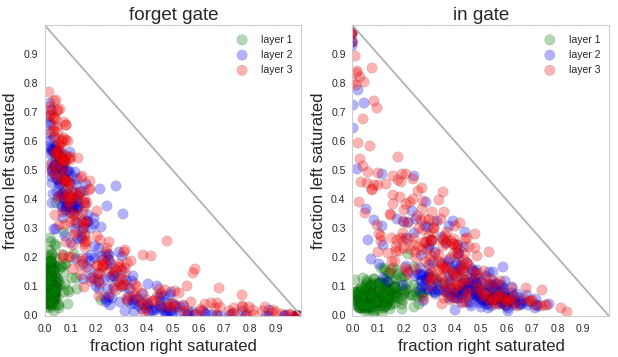
\includegraphics[width=0.6\textwidth]{newarchs/karpathy}
\caption[Saturations of 3-layer LSTM gates]{Saturation rates of 3-layer LSTM. The input gate modulates
the candidate update, while the forget gate is as defined in this chapter. Figure from
\autocite{Karpathy2016}, reproduced with permission.}
\label{fig:karpathy}
\end{figure}

It is also worth considering how this gating scheme affects the gradients during back-propagation.
In order to update the weights producing the gate signal, we will need the gradient of the hidden
state with respect to the gate signal itself at some earlier time \(i < t\):
\begin{align}
	\frac{\partial h_t}{\partial p_i} &= 
		\left(\prod_{k=i+1}^t \frac{\partial h_k}{\partial h_{k-1}}\right) 
			\frac{\partial h_i}{\partial p_i} \\
\end{align} by the chain rule. Differentiating equation~\ref{eq:forgetgate} appropriately we
get
\begin{align}
	\frac{\partial h_t}{\partial p_i} &= 
		\left(\prod_{k=i+1}^t p_k\right)
			h_{i-1}. \\
\end{align}
This makes it clear that the gating does not just happen during the forward pass. The gradients
continue to be gated in the same way as the states. This suggests the gate could struggle to
learn long time dependencies as information that is erroneously decayed during the forward pass
will have a similarly small contribution to the gradients.

Repeating the process with respect to the candidate activations, it is clear that precisely
the same argument applies.
\begin{align}
	\frac{\partial h_t}{\partial z_i} &= 
	\left(\prod_{k=i+1}^t \frac{\partial h_k}{\partial h_{k-1}}\right) 
			\frac{\partial h_i}{\partial z_i} \\
	&= \left(\prod_{k=i+1}^t p_k\right) \cdot
			1. \\
\end{align} During training this will be multiplied by the back-propagated error. If the gates
exhibit a strong decay, then candidate activation will also be forced to update primarily on
local information.

\subsubsection{Convex Gate}
In order to repeat the analysis with the convex gate, we need to more carefully define initial
conditions. In particular, let \(p_0 = 0\) and correspondingly \(h_0 = z_0\) be some initial
state.
\begin{align}
	h_0 &= z_0 \\
    h_1 &= p_1z_0 + (1-p_1)z_1 \\
    h_2 &= p_2p_1z_0 + p_2(1-p_1)z_1 + (1-p_2)z_2 \\
    h_3 &= p_3p_2p_1z_0 + p_3p_2(1-p_1)z_1 + p_3(1-p_2)z_2 + (1-p_3)z_3 \\
\end{align} giving rise to the general form
\begin{equation}
	h_t = \sum_{i=0}^t \left(\prod_{j=i+1}^t p_j\right) (1 - p_i) z_i
\end{equation} ensuring we define \(\prod_{j=i+1}^tp_j = 1\) if \(i = t\).
This is very close to what we had above, but the extra \(1-p_i\) in the
coefficients has significant impact. Firstly, we can prove the following statement which shows
that the sum over states is a convex sum.

\begin{prop} [Conservation of attention]
At any time \(t > 1\),
	\begin{equation} \label{eq:cvexforward}
		\sum_{i=0}^t \left(\prod_{j=i+1}^t p_j\right) (1 - p_i) = 1.
	\end{equation}
The coefficients of all previous states sum to one.
\label{prop:convexsum}
\end{prop}
\begin{proof}
If we expand the brackets, we can produce a telescoping sum. To ensure it telescopes
appropriately, we first pull the first and last terms out of the summation.
\begin{align}
    &\sum_{i=0}^t \left(\prod_{j=i+1}^t p_j\right) (1 - p_i) \\
    &= \prod_{j=1}^tp_j(1-p_0) + (1-p_t) + \sum_{i=1}^{t-1} \left(\prod_{j=i+1}^t p_j\right) (1 - p_i) \\
    &= \prod_{j=1}^tp_j(1-p_0) + (1-p_t) + \sum_{i=1}^{t-1} \left(\prod_{j=i+1}^t p_j\right) - \left(\prod_{j=i}^t p_j\right) \\
    &= \prod_{j=1}^tp_j(1-p_0) + (1-p_t) - \prod_{k=1}^t p_k + p_t \\
    &= \prod_{j=1}^tp_j - \prod_{k=1}^tp_k + 1 - p_0 + p_t - p_t \\
    &= 1
\end{align}
\end{proof}

Remarkably, this does not require \(p_i\) to be bounded at all. However, in order to compare
directly, we consider the common case when the gate signals
are between zero and one. The immediate effect of this lemma is that the scale of the states
depends only on the scale of the candidate activations. Each state is now a weighted mean of
past candidates, rather than a weighted sum.

Figure~\ref{fig:cvexgates} illustrates two of the possible shapes this can take. It is clear
that this gating scheme provides a different set of possible shapes to work with.
Specifically, if the gate mechanism starts outputting values very close to one, the window
applied to past states takes the form of a distinct spike over a small range of activations.
This occurs because if \(p_i\) is very close to one, \(1 - p_i\) is very close to zero, so
state \(h_{i-1}\) is going to be carried over with only a very minor contribution from
\(z_i\). Figure~\ref{fig:cvextrain} further emphasises the difference, making it clear that
the convex gate is capable of representing a fundamentally different set of window shapes
thant the forget gate, despite their similar formulation.

\begin{figure}[t]
\centering
\begin{subfigure}[t]{0.45\textwidth}
	\centering
	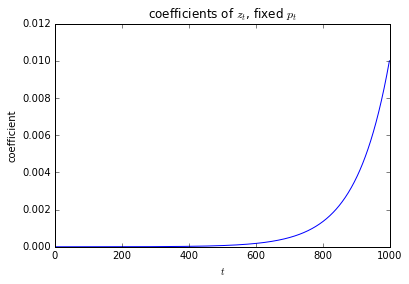
\includegraphics[width=\textwidth]{newarchs/cvexexp}
	\caption{Coefficients of \(z_t\) resulting from a fixed, high value of all \(p_t\)
	under the convex gate scheme.}
\end{subfigure}~
\begin{subfigure}[t]{0.45\textwidth}
	\centering
	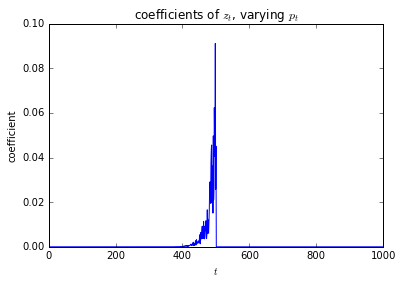
\includegraphics[width=\textwidth]{newarchs/cvexspike}
	\caption{Coefficients of \(z_t\) random \(p_t\) up to \(t=500\) and all \(p_t\) after
	500 set to 1.}
\end{subfigure}
\caption[Convex gate shapes]{Different window shapes produced by the convex gate.
 A simple adjustment to the formula
a much wider range of shapes.}
\label{fig:cvexgates}
\end{figure}

\begin{figure}[tbp]
\centering
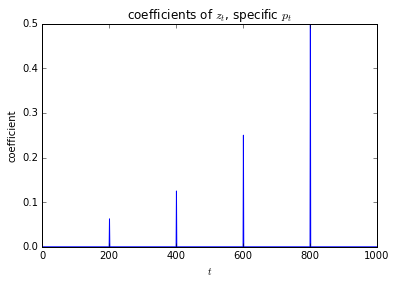
\includegraphics[width=0.45\textwidth]{newarchs/cvextrain}
\caption[Convex gate choosing several past candidates]
{Setting specific \(p_i\) to \(0.5\) picks out a set of past candidates, albeit with
an exponential decrease in their weighting.}
\label{fig:cvextrain}
\end{figure}

This enhanced range of window shapes makes these gates appealing as they may be able to reduce
interdependence between the gate mechanism and the candidate production mechanism. This might
allow us to remove the candidate's dependence on the previous state which should help solve the
potential instabilities noted above.

The downside of the system is that it may still struggle to learn long time dependencies early.
It would be straightforward to initialise the gate so that it has a mean activation of \(0.5\),
but this would correspond to an exponential decay of information. Unlike the forget gate simply
increasing the mean activation (for example by initialising the bias to a high positive value)
will not correspond to a flatter window.

To finish the analysis we consider again the gradients required for back-propagating error through
the gate. The gradient of the hidden state \(h_t\) with respect to a previous gate signal
\(p_i\) has the form:
\begin{align}
	\frac{\partial h_t}{\partial p_i} &= 
		\left(\prod_{k=i+1}^t \frac{\partial h_k}{\partial h_{k-1}}\right) 
			\frac{\partial h_i}{\partial p_i} \\
	&= \left( \prod_{k=i+1}^t p_k \right) (h_{i-1} - z_i) \label{eq:cvexgrad}
\end{align}
While the gradient of the state with respect to a prior candidate is
\begin{align}
	\frac{\partial h_t}{\partial z_i} &=
		\left(\prod_{k=i+1}^t \frac{\partial h_k}{\partial h_{k-1}}\right) 
			\frac{\partial h_i}{\partial z_i} \\
	&= \left( \prod_{k=i+1}^t p_k \right) (1 - p_i). \label{eq:cvexstategrad}
\end{align} The pattern here is fundamentally the same as the forget gate in that the gradient
is simply the coefficient assigned to \(z_i\) in the weighted sum that produced \(h_t\). Hence
all discussion of the differences in the gates' forward behaviour apply equally during the
backward pass.

Equation~\eqref{eq:cvexgrad} is interesting -- the gradient of the state with respect to the gate value
depends not just on the preceding state but on the difference between the state and the proposed
update. This suggests that during training what drives the updates is the possible changes that could be
made to the state, rather than just the state values itself. Meanwhile, equation~\eqref{eq:cvexstategrad}
shows that the ``conservation of attention'' in proposition~\ref{prop:convexsum} also applies on the
backward pass. This suggests that as long as the scale of the candidate activations are under control
there will be no problems with exploding gradients.


\subsubsection{Conclusions}
The convex gate by itself seems more capable than the forget gate as it is able to represent more
useful distributions over past candidate states. However, the combination of forget gate and input
gate employed in the LSTM are able to together represent the same behaviours, if not more. 
Despite this, we find the convex gate more appealing as it is provides the opportunity to design clean
and modular architectures in which each component has a precise role which does not overlap with others.



\section{Gated Tensor RNNs}
To design a gated RNN, there are three choices to make: how to gate the recurrence, how to compute
gate values and how to compute candidate updates. We are now in a position to make these choices on the
basis of chapter~\ref{C:tens} which discussed how to use tensors to model binary functions and
the above section~\ref{sec:gate} informs our choice of gate.



\subsection{Choices}
\subsubsection{Form of the gate}
We now consider how to compute the \(\vec{p}_i\) values.
The role of the gate is to manage the flow of new information into the states. The decisions it has to
make are whether to forget what is currently stored and completely overwrite it or reject a candidate
update if what is present in the state is somehow more useful. Of the two competing choices, we prefer
the convex gate. This is because it is capable of expressing a rich range of distributions over past
states in a single operation and without exploding gradients.
This gives a recurrence of the form
\begin{equation}\label{eq:propgate}
	\vec{h}_t = \vec{p}_t \odot \vec{h}_{t-1} + (\vec{1} - \vec{p}_t) \odot \vec{z}_t.
\end{equation}

\subsubsection{Gate calculation}
In order to decide whether incoming information should
overwrite the current state values, the gate will need to see the current values and the new information.
 The binary nature of this task suggests
the use of a tensor unit as discussed in chapter~\ref{C:tens}. Secondly if we want the full utility of
the convex gate, it seems logical to imbue it with full expressive power -- the bilinear tensor is a
perfect fit.

It is also necessary to choose a non-linearity. Much of the above analysis assumes the gate signals are
in the range \([0, 1]\) although this was not used in the proof of proposition~\ref{prop:convexsum}. The
typical approach is to ensure this smoothly with a sigmoid. Although sigmoids have undesirable
properties when used in feed-forward networks \autocite{Glorot2010} they remain the standard choice
when this kind of gating is desired \autocite{VandenOord2016, Oord2016} and we find no reason to
deviate from this.

The desired gate value is then calculated as:
\begin{equation}\label{eq:propgatevalue}
	\vec{p}_t = \sigma\left(\tran{\tilde{\vec{x}}}_t\widetilde{\tensor{W}}\tilde{\vec{h}}_{t-1} \right).
\end{equation}

Following the results in chapter~\ref{C:tens} we intend to represent the tensor in a CP decomposition.
It remains a choice to decide how to deal with the biases -- in the following experiments we tend to
include results for both choices for comparison. In particular, keeping the biases implicit potentially
provides the ability to regularise the model by restricting the rank, although it needs to be seen
empirically whether this affects adversely the representative power of the model.

Using a tensor in this fashion provides an interesting possibility: the ability to write to the memory
associatively. One interpretation of the tensor product is that it computes similarity measures between
its inputs. Under this interpretation, the gate is constantly computing weighted similarities between
the input and the current state. It is possible then for the gate to react if a certain pattern in the
input matches a pattern stored in the state and admit or deny a corresponding update. This example
shows the power of incorporating multiplicative connections -- this mode of behaviour is very difficult
to realise when the inputs share only an additive connection.

\subsubsection{Candidate update}
All that remains is to determine how to derive a candidate state update. In all of the architectures
surveyed apart from the Strongly Typed variants \autocite{Balduzzi2016} it is assumed that this needs
to be a binary function of the current input and the previous hidden state. Intuitively this needs to
be the case with the LSTM style forget gate, but as we have decided against that it is worth questioning
this assumption.

Removing this step makes each role in the network clearly defined. As each input comes in, it is
embedded into the state space. The gate decides whether it is important information and the state is
updated additively. The candidate production mechanism only needs to behave in as a feature
detector, transforming the input into a representation that captures its essential structure in a way
amenable to additive composition.

This scheme is appealing due to its simplicity and separation of
roles, although two questions remain to be answered: how does this affect the expressive power of the
network and how should we compute the necessary representation. The former is likely to be a best
answered empirically, although we make a brief note here. One aspect of the GRU and LSTM that is
certainly lost is what we term the ``carousel'' behaviour. A method for these networks to maintain
information in their hidden states for long time periods is for the candidate production mechanism to
learn an identity mapping from hidden states to hidden states. This behaviour is impossible to realise
unless the candidate state depends on the previous hidden state. Note that this is also the only way
that the Vanilla RNN can remember information for long time periods. Given the failures of the
Vanilla RNN, we hypothesise that removing this mode of behaviour should be no great loss. Further,
we suggest it may help optimisation if there is only one clear way in which to store information. This
leads us to conclude that we want to remove the hidden state from the candidate calculation.

What remains is to determine how to compute the candidate from the input. We wish to model a unary
mapping from the input to the candidate, so a logical way to proceed is with a standard feed-forward
layer:
\begin{equation}\label{eq:propcandidate}
	\vec{z}_t = f(\mat{W}_{in}\vec{x}_t + \vec{b}_{in}).
\end{equation} We experimented with a number of options for the non-linearity \(f\) and found the best
performance was consistently achieved with either a linear rectifier \(\rho(x) = \max(0, x)\) or no
non-linearity at all. This echoes trends in feed-forward networks away from saturating non-linearities
towards unbounded, piecewise linear activation functions \autocite{Goodfellow2013, He}. It is
interesting that for many tasks a completely linear candidate performed optimally -- the only hypothesis
is that the sigmoid applied to the gate is enough non-linearity to preserve the representative power of
the network as a whole and that a linear layer will have very strong gradients and potentially
preferable training dynamics \autocite{Saxe2013}.

While a single feed-forward layer was sufficient in our experiments, there is scope to expand this,
potentially in a task-dependent manner. For example this could be a deeper feed-forward architecture,
a convolutional neural network if the inputs have appropriate structure or even an identity map if the
input to the network is already high-level features.

\subsection{Tensor Gate Unit}
Bringing together equations \eqref{eq:propgate}, \eqref{eq:propgatevalue} and \eqref{eq:propcandidate}
gives us the proposed Tensor Gate Unit (TGU) which computes its hidden states as follows:
\begin{align}\label{eq:tgu}
	\vec{h}_t &= \vec{p}_t \odot \vec{h}_{t-1} + (\vec{1}-\vec{p}_t)\vec{z}_t \\
	\vec{p}_t &= \sigma\left(\tran{\tilde{\vec{x}}}_t\widetilde{\tensor{W}}\tilde{\vec{h}}_{t-1} \right)\\
	\vec{z}_t &= f(\mat{W}_{in}\vec{x}_t + \vec{b}_{in})
\end{align}

We will represent the tensor with a CP decomposition. We still have to decide whether to incorporate the
biases in the decomposition or keep them separate. A straightforward inclination is to keep them separate
for the reasons outlined in section~\ref{sec:gmrnn}, leading to the following gate equation:
\begin{align}\label{eq:tggateseparate}
	\vec{d}_t &= \tran{\mat{B}}\left(\mat{A}\vec{x}_t\odot\mat{C}\vec{h}_{t-1}\right)\\
	\vec{p}_t &= \sigma\left(
		\vec{d}_t
		+ \mat{U}\vec{h}_{t-1} + \mat{V}\vec{x}_t + \vec{b}\right).
\end{align}
We also consider the alternative where the bias matrices are folded into the decomposition:
\begin{align}\label{eq:tggatecombined}
	\vec{d}_t &= \tran{\mat{B}}\left((\mat{A}\vec{x}_t 
	+ \vec{b}_x)\odot(\mat{C}\vec{h}_{t-1} + \vec{b}_h)\right)\\
	\vec{p}_t &= \sigma(\vec{d}_t)
\end{align}
